\chapter{Android Malware Obfuscators}

\section{Android Malware Detectors}
With the rise of the Android Operating systems, the amount of malware associated with it has also risen significantly. From a market share of 2.8 \% in 2009 \cite{androidShare2009} , Android captured about 75\% of the market in 2012 \cite{androidShare2009}. As shown in fig.~\ref{osMarketShare} , we can see that the growth and adoption of Android has been very steep. This rapid proliferation of Android resulted in an equally rapid rise of Android malware.

  \vspace{3mm}
  \begin{center}
  	%\centering
  	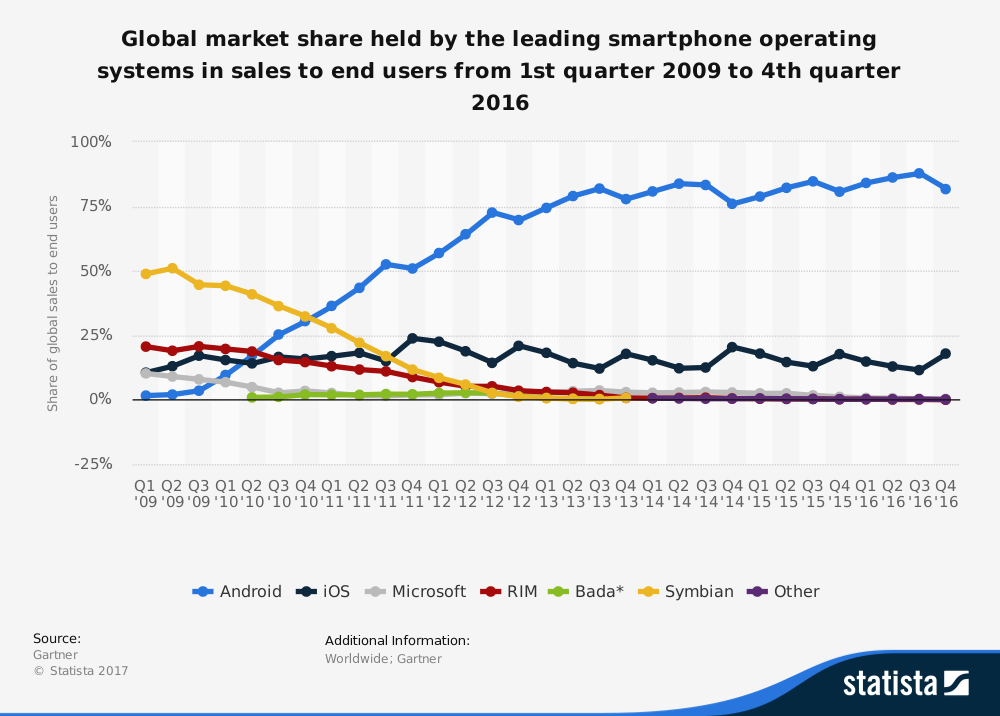
\includegraphics[width=0.8\textwidth]{OS_Market_Share.png}
  	\captionof{figure}{Market Share of mobile operating systems}
  	\label{osMarketShare}
  \end{center}
  \vspace{3mm}
  
  
   \vspace{3mm}
   \begin{center}
   	%\centering
   	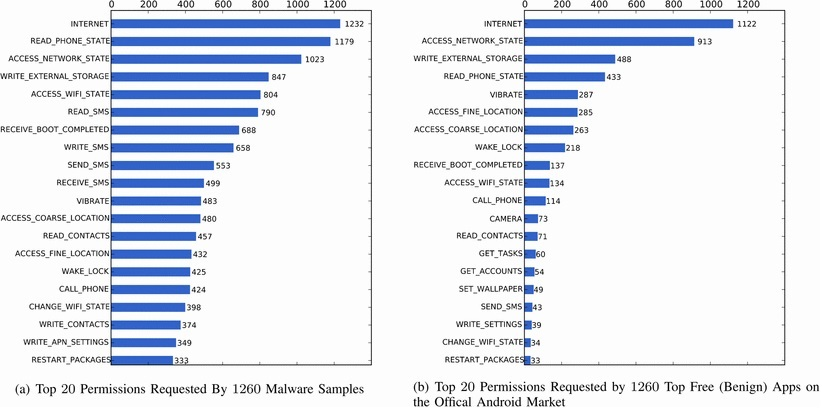
\includegraphics[width=0.8\textwidth]{permissionsList1.png}
   	\captionof{figure}{Top 20 permissions in Android in 2012}
   	\label{permissionsAndroid}
   \end{center}
   \vspace{3mm}
   
With the increase in the number of Android malware being released to the wild, their level of sophistication also increased. Android malware detectors used the number of permissions requested by an app to determine its legitimacy. As shown in the fig. ~\ref{permissionsAndroid} obtained from \cite{zhou}, we can see that benign and malicious Android applications have access requests that are very similar.

Due to this, using access requests as a measure for classifying android applications became ineffective. The various types of Android malware can be broadly classified into the following categories, depending on the type of malicious activities they perform \cite{zhou}:

\begin{itemize}
	\item Privilege Escalation
	\item Remote Control
	\item Monetary Loss
	\item Information Collection
\end{itemize}

\subsection{Privilege Escalation}
In this type of attack, the malicious app that is installed on a device, attempts to grant itself additional privileges than the one it requires. This is achieved by using known exploits in the Android operating system.
\subsection{Remote Control}
A very high percentage of malware attempts to use the compromised device as a remote bot. In some malware families, the remote URL that is being used to control the device. Such encryption makes it very difficult to detect these types of malware and this will be a primary area of focus in this thesis.
\subsection{Monetary Loss}
A very direct way of monetizing malware is to make unsuspecting users subscribe to services that cost a lot of money. Such services are run by the malware perpetrators and will enable them to charge the infected devices' owners money for services that they are not aware of. To achieve this, some malware use the remote control to push down numbers of services to the devices and then enroll them.
\subsection{Information Collection}
Many malware programs attempt to collect the personal information of users. Such personally identifiable information makes it easy for scamsters to dupe people using various other schemes. Malware belonging to this family tries to steal personal information of the compromised device's owner, as well as the details of people in their contact lists. This information is then sold through different means to interested parties.

\section{Android Malware Detection Limitations}
One of the major limitation of malware detection in Android is the limited processing power of the devices running Android. Due to processing and memory constraints, generic malware detection has to be restricted to static analysis techniques. In general, all the existing Android security solutions can be classified into \em{Static Analysis} and \em{Dynamic Analysis} \cite{arshad}.

\subsection{Static Analysis}
Static Analysis is a technique in which the an application is evaluated for its trustworthiness by disassembling and checking its source code. The application is not executed for this analysis. 
\subsubsection{Signature Based Detection}
Signature based detection is a type of static analysis technique. In this method, a virus is examined by extracting its signature and then comparing it with signatures from known malware. The limitation of this technique is that it is incapable of detecting unknown malware types. The signatures of known malware are stored in a signature database. In addition to this, the signature database also requires that it is updated constantly. Without an up-to-date signature database, most of the prevalent malware could slip through undetected. This is difficult in the case of Android Malware detectors as the device possess limited memory and it would be infeasible to store all virus definitions on the device. If the virus definitions were to be moved to a remote server, it would use up considerable amount of data traffic for performing the validation. These are some serious limitations that hinder traditional signature matching techniques.
\subsubsection{Permission Based Detection}
This is a straightforward approach to detecting malware in Android systems. In this method, the number of permissions an application requires is used to determine its classification as a malicious or a benign file. Some research has been done in this area wherein the Android Manifest file is analyzed for extracting information\cite{sato} about the permissions requested by the application. This information is used to assign a score of relevancy to the permissions requested. This score is then compared against a threshold for determining the malicious intent of an app. There are variations to this technique and some methods yield better results than the others. This method is a very quick way of determining the malicious nature of applications. But a serious limitation of this method is that it does not analyze the source code or the working of the app. Only the Manifest file is analyzed. A lot of malware apps use permissions similar to the benign apps. Hence, permissions based detection should be used in conjuction with a second confirmation method to validate an app.
\subsection{Dynamic Analysis}
In this method, the application is executed and it is analyzed during the runtime. It becomes very easy to identify sections of code or execution blocks that were missed during the static analysis of an application. Dynamic analysis methods are also effective against obfuscation and encryption techniques.
\subsubsection{Anomaly Based Detection}
An application is executed and the system calls generated by it are recorded in a log. This log is then sent for analysis to a remote server, where the various behavior of malware are recorded. Using that as a basis, the log files are analyzed, and the results are aggregated. This result, in collaboration with other techniques are used to classify the file as malicious or not.
\subsubsection{Emulation Technique}
Yan et al. \cite{yan} propose a technique in which a Virtual machine is used to analyze an application. In common virtual machine based detection techniques, the anti-malware program and the malware execute in the same environment. This makes them detectable to each other. In the platform presented by Yan et al. \cite{yan}, the antimalware, \emph{DroidScope}, stays out  of the execution environment and monitors the execution as a whole. This enables it to detect the malware without being detected by the malware.